%%
%% Copyright (C) 2008  Distributed Computing System (DCS) Group, Computer
%% Science Department - University of Piemonte Orientale, Alessandria (Italy).
%%
%% This program is free software: you can redistribute it and/or modify
%% it under the terms of the GNU Lesser General Public License as published
%% by the Free Software Foundation, either version 3 of the License, or
%% (at your option) any later version.
%%
%% This program is distributed in the hope that it will be useful,
%% but WITHOUT ANY WARRANTY; without even the implied warranty of
%% MERCHANTABILITY or FITNESS FOR A PARTICULAR PURPOSE.  See the
%% GNU Lesser General Public License for more details.
%%
%% You should have received a copy of the GNU Lesser General Public License
%% along with this program.  If not, see <http://www.gnu.org/licenses/>.
%%

\section{Esecuzione} \label{sec:exec}

In questa sezione verranno mostrati i passi base per effettuare il ``rendering'' di una semplice scena 3D tramite l'applicazione \mgTheApp{}.

Prima di eseguire l'applicazione \mgTheApp{}, assicurarsi che lo ``scheduler'' \emph{mygrid} sia in esecuzione; per maggiori dettagli su come eseguire ``mygrid'', si consulti la guida presente sul sito ufficiale di \emph{OurGrid} o le istruzioni pubblicate sul sito di \emph{ShareGrid}.

\subsection{Scena: \emph{VictorDancing}} \label{ssec:exec-victor}

La scena presentata in questa sezione \`e tratta dalla sezione \emph{Animation} del libro \emph{ActionBook} \cite{Krizanovskij2007ActioBook}; l'animazione risultante, composta da $24$ ``frame'', dovrebbe rappresentare una creatura, dalle sembianze umane, che danza.
Il file della scena \`e presente nella sotto-cartella \mgCode{examples} della directory in cui \`e stata installata l'applicazione \mgTheApp{}.
Il ``rendering'' viene effettuato tramite una suddivisione in $5$ gruppi da $5$ ``frame'' (fatta eccezione per l'ultimo gruppo, composto da $4$ ``frame'').
I file ottenuti dal ``rendering'' di ogni gruppo di ``frame'' rappresentano delle animazioni in formato AVI.

Verranno ora elencati i passi per effettuare il ``rendering'' di questa scena tramite \mgTheApp{}.
\begin{enumerate}
\item Esegure l'applicazione \mgTheApp{} attraverso lo script di esecuzione \mgTheAppFile{.sh}
\begin{mgCodeBox}
\small
./\mgTheAppFile{.sh}
\end{mgCodeBox}
\item Dal menu:
\begin{mgCodeBox}
\small
\#\#\# Sharegrid Grid Renderer \#\#\#\newline
--- Main Menu:\newline
1. Insert a new job\newline
8. About\newline
9. Exit\newline
? 
\end{mgCodeBox}
Digitare il valore $1$.
\item Apparir\`a il menu che permette di inserire le informazioni sulla scena su cui effettuare il ``rendering'': digitare il valore $1$, per inserire il nome della scena, e premere il tasto \mgCode{Invio}:
\begin{mgCodeBox}
\small
\#\#\# Job selection \#\#\#\newline
--- New job\newline
1. Scene name\ \ \ \ \ \ \ \ \ \ \ \ \ \{ \}\newline
2. Scene file\ \ \ \ \ \ \ \ \ \ \ \ \ \{ \} [*]\newline
3. First frame\ \ \ \ \ \ \ \ \ \ \ \ \{ \}\newline
4. Last frame\ \ \ \ \ \ \ \ \ \ \ \ \ \{ \}\newline
5. Step frame\ \ \ \ \ \ \ \ \ \ \ \ \ \{ \}\newline
6. Input files\ \ \ \ \ \ \ \ \ \ \ \ \{ \}\newline
98. Review job settings\newline
99. Back to previous menu\newline
(---\newline
 Informations marked with:\newline
 - '[*]' are mandatory\newline
 - '\{X\}' have been already inserted by the user\newline
---)\newline
? \textbf{1}
\end{mgCodeBox}
\item Verr\`a richiesto di inserire il nome della scena; il programma offre, come valore di default, la stringa \mgCode{user-blender\_20070928\_1407}; scrivere, invece, la stringa \mgCode{VictorDancing} e premere il tasto \mgCode{Invio}:
\begin{mgCodeBox}
\small
\{Scene name>> Symbolic name used for identifying the scene [user-blender\_20070928\_1407]? \textbf{VictorDancing}
\end{mgCodeBox}
\item Apparir\`a nuovamente il menu relativo ai dati della scena; digitare il valore $2$, per inserire il percorso al file della scena, e premere il tasto \mgCode{Invio}:
\begin{mgCodeBox}
\small
\#\#\# Job selection \#\#\#\newline
--- New job\newline
1. Scene name\ \ \ \ \ \ \ \ \ \ \ \ \ \{X\}\newline
2. Scene file\ \ \ \ \ \ \ \ \ \ \ \ \ \{ \} [*]\newline
3. First frame\ \ \ \ \ \ \ \ \ \ \ \ \{ \}\newline
4. Last frame\ \ \ \ \ \ \ \ \ \ \ \ \ \{ \}\newline
5. Step frame\ \ \ \ \ \ \ \ \ \ \ \ \ \{ \}\newline
6. Input files\ \ \ \ \ \ \ \ \ \ \ \ \{ \}\newline
98. Review job settings\newline
99. Back to previous menu\newline
(---\newline
 Informations marked with:\newline
 - '[*]' are mandatory\newline
 - '\{X\}' have been already inserted by the user\newline
---)\newline
? \textbf{2}
\end{mgCodeBox}
\item Verr\`a richiesto di inserire il percorso al file della scena; il programma offre, come valore di default il file \mgCode{user-blender\_20070928\_1407}; scrivere, invece, la stringa \mgCode{./examples/data/blender/VictorDancing.blend} e premere il tasto \mgCode{Invio}:
\begin{mgCodeBox}
\small
\{Scene file>> Path to the scene file [user-blender\_20070928\newline
\_1407.blend]?  \textbf{./examples/data/blender/VictorDancing.blend}
\end{mgCodeBox}
\item \label{lbl:exec-victor-startframe-useless} Apparir\`a nuovamente il menu relativo ai dati della scena; digitare il valore $3$, per inserire il numero del primo ``frame'' da sottoporre al ``rendering'', e premere il tasto \mgCode{Invio}:
\begin{mgCodeBox}
\small
\#\#\# Job selection \#\#\#\newline
--- New job\newline
1. Scene name\ \ \ \ \ \ \ \ \ \ \ \ \ \{X\}\newline
2. Scene file\ \ \ \ \ \ \ \ \ \ \ \ \ \{X\} [*]\newline
3. First frame\ \ \ \ \ \ \ \ \ \ \ \ \{ \}\newline
4. Last frame\ \ \ \ \ \ \ \ \ \ \ \ \ \{ \}\newline
5. Step frame\ \ \ \ \ \ \ \ \ \ \ \ \ \{ \}\newline
6. Input files\ \ \ \ \ \ \ \ \ \ \ \ \{ \}\newline
98. Review job settings\newline
99. Back to previous menu\newline
(---\newline
 Informations marked with:\newline
 - '[*]' are mandatory\newline
 - '\{X\}' have been already inserted by the user\newline
---)\newline
? \textbf{3}
\end{mgCodeBox}
\item \label{lbl:exec-victor-startframe2-useless} Verr\`a richiesto di inserire il numero del primo ``frame'' da cui iniziare il ``rendering'' della scena; il programma offre, come valore di default il valore $1$; accettare tale valore premendo il tasto \mgCode{Invio} (senza immettere alcun valore):
\begin{mgCodeBox}
\small
\{Start frame>> Number of the first frame of the scene to be rendered [1]?
\end{mgCodeBox}
\item Apparir\`a nuovamente il menu relativo ai dati della scena; digitare il valore $4$, per inserire il numero dell'ultimo ``frame'' da sottoporre al ``rendering'', e premere il tasto \mgCode{Invio}:
\begin{mgCodeBox}
\small
\#\#\# Job selection \#\#\#\newline
--- New job\newline
1. Scene name\ \ \ \ \ \ \ \ \ \ \ \ \ \{X\}\newline
2. Scene file\ \ \ \ \ \ \ \ \ \ \ \ \ \{X\} [*]\newline
3. First frame\ \ \ \ \ \ \ \ \ \ \ \ \{X\}\newline
4. Last frame\ \ \ \ \ \ \ \ \ \ \ \ \ \{ \}\newline
5. Step frame\ \ \ \ \ \ \ \ \ \ \ \ \ \{ \}\newline
6. Input files\ \ \ \ \ \ \ \ \ \ \ \ \{ \}\newline
98. Review job settings\newline
99. Back to previous menu\newline
(---\newline
 Informations marked with:\newline
 - '[*]' are mandatory\newline
 - '\{X\}' have been already inserted by the user\newline
---)\newline
? \textbf{4}
\end{mgCodeBox}
\item Verr\`a richiesto di inserire il numero dell'ultimo ``frame'' in cui terminare il ``rendering'' della scena; il programma offre, come valore di default il valore assunto dal primo ``frame'', in questo caso il valore $1$; digitare il valore $24$ e premere il tasto \mgCode{Invio}:
\begin{mgCodeBox}
\small
\{End frame>> Number of the last frame of the scene to be rendered [1]? \textbf{24}
\end{mgCodeBox}
\item Apparir\`a nuovamente il menu relativo ai dati della scena; digitare il valore $5$, per inserire il numero di ``frame'' da includere in ciascun gruppo, e premere il tasto \mgCode{Invio}:
\begin{mgCodeBox}
\small
\#\#\# Job selection \#\#\#\newline
--- New job\newline
1. Scene name\ \ \ \ \ \ \ \ \ \ \ \ \ \{X\}\newline
2. Scene file\ \ \ \ \ \ \ \ \ \ \ \ \ \{X\} [*]\newline
3. First frame\ \ \ \ \ \ \ \ \ \ \ \ \{X\}\newline
4. Last frame\ \ \ \ \ \ \ \ \ \ \ \ \ \{X\}\newline
5. Step frame\ \ \ \ \ \ \ \ \ \ \ \ \ \{ \}\newline
6. Input files\ \ \ \ \ \ \ \ \ \ \ \ \{ \}\newline
98. Review job settings\newline
99. Back to previous menu\newline
(---\newline
 Informations marked with:\newline
 - '[*]' are mandatory\newline
 - '\{X\}' have been already inserted by the user\newline
---)\newline
? \textbf{5}
\end{mgCodeBox}
\item Verr\`a richiesto di inserire il numero di ``frame'' da includere in ciascuna partizione della scena; il programma offre, come valore di default il valore $25$; digitare il valore $5$ e premere il tasto \mgCode{Invio}:
\begin{mgCodeBox}
\small
\{Step frame>> Number of contiguous frames the scene will be subdivided [25]? \textbf{5}
\end{mgCodeBox}
\item Apparir\`a nuovamente il menu relativo ai dati della scena; dato che la scena non necessita di ulteriori risorse addizionali, la voce numero $6$ del menu verr\`a saltata. Digitare il valore $98$, per visualizzare il riepilogo delle informazioni inserire, e premere il tasto \mgCode{Invio}:
\begin{mgCodeBox}
\small
\#\#\# Job selection \#\#\#\newline
--- New job\newline
1. Scene name\ \ \ \ \ \ \ \ \ \ \ \ \ \{X\}\newline
2. Scene file\ \ \ \ \ \ \ \ \ \ \ \ \ \{X\} [*]\newline
3. First frame\ \ \ \ \ \ \ \ \ \ \ \ \{X\}\newline
4. Last frame\ \ \ \ \ \ \ \ \ \ \ \ \ \{X\}\newline
5. Step frame\ \ \ \ \ \ \ \ \ \ \ \ \ \{X\}\newline
6. Input files\ \ \ \ \ \ \ \ \ \ \ \ \{ \}\newline
98. Review job settings\newline
99. Back to previous menu\newline
(---\newline
 Informations marked with:\newline
 - '[*]' are mandatory\newline
 - '\{X\}' have been already inserted by the user\newline
---)\newline
? \textbf{98}
\end{mgCodeBox}
\item Verranno visualizzate le seguenti informazioni:
\begin{mgCodeBox}
\small
Scene name: VictorDancing\newline
Scene file: ./examples/data/blender/VictorDancing.blend\newline
Start frame number: 1\newline
End frame number: 24\newline
Step frame number: 5\newline
Input files:  <none>\newline
\end{mgCodeBox}
\item Apparir\`a nuovamente il menu relativo ai dati della scena. Digitare il valore $99$, per ritornare al menu principale, e premere il tasto \mgCode{Invio}:
\begin{mgCodeBox}
\small
\#\#\# Job selection \#\#\#\newline
--- New job\newline
1. Scene name\ \ \ \ \ \ \ \ \ \ \ \ \ \{X\}\newline
2. Scene file\ \ \ \ \ \ \ \ \ \ \ \ \ \{X\} [*]\newline
3. First frame\ \ \ \ \ \ \ \ \ \ \ \ \{X\}\newline
4. Last frame\ \ \ \ \ \ \ \ \ \ \ \ \ \{X\}\newline
5. Step frame\ \ \ \ \ \ \ \ \ \ \ \ \ \{X\}\newline
6. Input files\ \ \ \ \ \ \ \ \ \ \ \ \{ \}\newline
98. Review job settings\newline
99. Back to previous menu\newline
(---\newline
 Informations marked with:\newline
 - '[*]' are mandatory\newline
 - '\{X\}' have been already inserted by the user\newline
---)\newline
? \textbf{99}
\end{mgCodeBox}
\item Apparir\`a il menu iniziale, arricchito di nuove informazioni; a questo punto \`e possibile ritornare al menu dei dati della scena per modificare le informazioni appena inserite (voce numero $2$ del menu), eseguire il ``rendering'' distribuito della scena (voce numero $3$ del menu), esportare su un file i dati appena inseriti (voce numero $4$ del menu) oppure inserire una nuova scena, sostituiendo i dati appena inseriti (voce del menu $1$).
Supponendo di voler lanciare il ``rendering'' della scena, digitare il valore $3$ e premere il tasto \mgCode{Invio}:
\begin{mgCodeBox}
\small
\#\#\# Sharegrid Grid Renderer \#\#\#\newline
--- Main Menu:\newline
1. Insert a new job\newline
2. Modify current job\newline
3. Execute current job\newline
4. Export current job\newline
8. About\newline
9. Exit\newline
? \textbf{3}
\end{mgCodeBox}
\item L'applicazione \mgTheApp{} contatter\`a lo ``scheduler'' \emph{mygrid}.
\begin{itemize}
\item Se l'interazione con ``mygrid'' ha successo verr\`a visualizzato il messaggio di conferma:
\begin{mgCodeBox} 
\small
\textcolor{green}{[OK] Job successfully submitted.}\newline
\textcolor{blue}{[INFO] The job execution identifier is: 1}\newline
\textcolor{blue}{[INFO] Use this identifier for retrieving job\newline
execution information or for cancelling the job\newline
execution.}
\end{mgCodeBox} 
\item Se ``mygrid'' non \`e in esecuzione verr\`a visualizzato il messaggio di errore:
\begin{mgCodeBox}
\small
\textcolor{red}{[ERROR] Current job cannot be executed. Please, check if the scheduler is running!}
\end{mgCodeBox}
Per risolvere il problema, \`e sufficiente eseguire l'applicazione \emph{mygrid} (non \`e necessario uscire dall'applicazione \mgTheApp{}) e digitare nuovamente il valore $3$ per tentare l'esecuzione.
\end{itemize}
\item Il valore indicato come \emph{job execution identifier}, restituito quando \mgTheApp{} riesce a sottomettere con successo, a \emph{mygrid}, le istruzioni per il ``rendering'', pu\`o essere utilizzato sia all'interno di \mgTheApp{} per ottenere informazioni sullo stato di esecuzione o per annullare l'esecuzione, sia attraverso l'interfaccia testuale o grafica di \emph{mygrid}. Per esempio, per visualizzare lo stato di esecuzione, digitare il valore $1$ e premere il tasto \mgCode{Invio}:
\begin{mgCodeBox}
\small
\#\#\# Job execution \#\#\#\newline
1. Execution status\newline
2. Cancel execution\newline
3. Execute again\newline
4. Monitor execution\newline
9. Back to previous menu\newline
? \textbf{1}
\end{mgCodeBox}
\item Verr\`a visualizzato un messaggio indicante lo stato di esecuzione del ``rendering''; per esempio, il messaggio:
\begin{mgCodeBox}
\small
\textcolor{blue}{[INFO] The execution IDENTIFIER of the job is: 1}\newline
\textcolor{blue}{[INFO] The execution STATUS of the job is: RUNNING}
\end{mgCodeBox}
informa che il ``rendering'', con ``job execution identifier'' pari a $1$, \`e attualmente in esecuzione (\mgCode{RUNNING}).
\item \`E inoltre possibile osservare lo stato di esecuzione del job in modo interattivo attraverso un'interfaccia grafica; per eseguire tale interfaccia, digitare il valore $4$ e premere il tasto \mgCode{Invio}:
\begin{mgCodeBox}
\small
\#\#\# Job execution \#\#\#\newline
1. Execution status\newline
2. Cancel execution\newline
3. Execute again\newline
4. Monitor execution\newline
9. Back to previous menu\newline
? \textbf{4}
\end{mgCodeBox}
\item Verr\`a visualizzato un messaggio di conferma di esecuzione del monitor di job:
\begin{mgCodeBox}
\small
\textcolor{green}{[OK] Job monitor has been successfully started.}
\end{mgCodeBox}
e apparir\`a una finestra indicante lo stato di esecuzione del ``rendering'' di ogni gruppo di ``frame'' in cui il ``rendering'' dell'intera scena \`e stato scomposto (Fig.~\ref{fig:monitor-victor}).
\begin{figure}
\centering
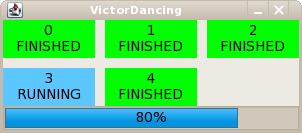
\includegraphics{images/victor_monitor}
\caption{Monitor dello stato di esecuzione del ``rendering'' di ogni gruppo di ``frame''.}
\label{fig:monitor-victor}
\end{figure}
\item Una volta che lo stato di esecuzione del ``rendering'' diventa \mgCode{FINISHED}, uscire dal programma digitando il valore $9$, seguito dal tasto \mgCode{Invio}, e, nuovamente, il valore $9$, seguito dal tasto \mgCode{Invio}.
\item All'interno della cartella da cui \mgTheApp{} \`e stato eseguito, si troveranno $5$ file in formato ZIP:
\begin{mgCodeBox}
\small
VictorDancing.blend-rendered.zip\_1\_5\newline
VictorDancing.blend-rendered.zip\_6\_10\newline
VictorDancing.blend-rendered.zip\_11\_15\newline
VictorDancing.blend-rendered.zip\_16\_20\newline
VictorDancing.blend-rendered.zip\_21\_24
\end{mgCodeBox}
\item Scompattare ciascun file all'interno di una opportuna cartella; la scompattazione creer\`a la sotto-cartella \mgCode{VictorDancing.blend-rendered} in cui si troveranno i seguenti file:
\begin{mgCodeBox}
\small
0001\_0005.avi\newline
0006\_0010.avi\newline
0011\_0015.avi\newline
0016\_0020.avi\newline
0021\_0024.avi
\end{mgCodeBox}
\item \`E ora possibile combinare i suddetti file in modo opportuno o, semplicemente, visualizzare la scena, per esempio, con il comando:
\begin{mgCodeBox}
\small
blender -a 0001\_0005.avi 0006\_0010.avi 0011\_0015.avi\newline
0016\_0020.avi 0021\_0024.avi
\end{mgCodeBox}
In Fig.~\ref{fig:exec-victor} sono mostrati alcuni fotogrammi della scena.
\end{enumerate}
Si noti che, durante l'immissione dei dati relativi alla scena, non \`e necessario inserire tutte le informazioni; in particolare, quando si accetta il valore di default proposto da \mgTheApp{} , \`e possibile evitare di accedere alla relativa voce di menu.
Ne segue che, in questo esempio, i passi descritti ai punti \ref{lbl:exec-victor-startframe-useless} e \ref{lbl:exec-victor-startframe2-useless} possono essere evitati.
Ci\`o non vale, per\`o, se la voce del menu \`e etichettata con il simbolo \mgCode{[*]} (come nel caso del file della scena), il quale indica che l'inserimento del valore \`e obbligatorio.

\begin{figure}
\centering
\begin{minipage}[t]{0.22\linewidth}
\centering

\includegraphics[scale=0.30]{images/victor-1}
\end{minipage}
\hspace{0.3cm}
\begin{minipage}[t]{0.22\linewidth}
\centering

\includegraphics[scale=0.30]{images/victor-2}
\end{minipage}
\hspace{0.3cm}
\begin{minipage}[t]{0.22\linewidth}
\centering

\includegraphics[scale=0.30]{images/victor-3}
\end{minipage}
\hspace{0.3cm}
\begin{minipage}[t]{0.22\linewidth}
\centering

\includegraphics[scale=0.30]{images/victor-4}
\end{minipage}
\caption{Alcuni fotogrammi della scena \emph{VictorDancing}.}
\label{fig:exec-victor}
\end{figure}

\subsection{Scena: \emph{ArrayDemo}} \label{ssec:exec-arraydemo}

La scena presentata in questa sezione \`e tratta dalla sezione \emph{animation} dei test di regressione di \emph{Blender} (scena \emph{array3.blend}); l'animazione risultante, composta da $737$ ``frame'', dovrebbe rappresentare un vettore di cubi che effettuano una serie di rotazioni e traslazioni.
Il file della scena \`e presente nella sotto-cartella \mgCode{examples} della directory in cui \`e stata installata l'applicazione \mgTheApp{}.
Il ``rendering'' viene effettuato tramite una suddivisione in $30$ gruppi da $25$ ``frame'' (fatta eccezione per l'ultimo gruppo, composto da $12$ ``frame'').
A differenza della scena presentata nella sezione precedente, i file prodotti in output dal ``rendering'' di ogni gruppo di ``frame'' sono delle immagini in formato PNG.
Per ottenere il file di animazione finale, \`e necessario che nel sistema sia installato l'applicativo \emph{ffmpeg}.

Verranno ora elencati i passi per effettuare il ``rendering'' di questa scena tramite \mgTheApp{}.
\begin{enumerate}
\item Esegure l'applicazione \mgTheApp{} attraverso lo script di esecuzione \mgTheAppFile{.sh}
\begin{mgCodeBox}
\small
./\mgTheAppFile{.sh}
\end{mgCodeBox}
\item Dal menu:
\begin{mgCodeBox}
\small
\#\#\# Sharegrid Grid Renderer \#\#\#\newline
--- Main Menu:\newline
1. Insert a new job\newline
8. About\newline
9. Exit\newline
? 
\end{mgCodeBox}
Digitare il valore $1$.
\item Apparir\`a il menu che permette di inserire le informazioni sulla scena su cui effettuare il ``rendering'': digitare il valore $1$, per inserire il nome della scena, e premere il tasto \mgCode{Invio}:
\begin{mgCodeBox}
\small
\#\#\# Job selection \#\#\#\newline
--- New job\newline
1. Scene name\ \ \ \ \ \ \ \ \ \ \ \ \ \{ \}\newline
2. Scene file\ \ \ \ \ \ \ \ \ \ \ \ \ \{ \} [*]\newline
3. First frame\ \ \ \ \ \ \ \ \ \ \ \ \{ \}\newline
4. Last frame\ \ \ \ \ \ \ \ \ \ \ \ \ \{ \}\newline
5. Step frame\ \ \ \ \ \ \ \ \ \ \ \ \ \{ \}\newline
6. Input files\ \ \ \ \ \ \ \ \ \ \ \ \{ \}\newline
98. Review job settings\newline
99. Back to previous menu\newline
(---\newline
 Informations marked with:\newline
 - '[*]' are mandatory\newline
 - '\{X\}' have been already inserted by the user\newline
---)\newline
? \textbf{1}
\end{mgCodeBox}
\item Verr\`a richiesto di inserire il nome della scena; il programma offre, come valore di default, la stringa \mgCode{user-blender\_20080314\_1634}; scrivere, invece, la stringa \mgCode{ArrayDemo} e premere il tasto \mgCode{Invio}:
\begin{mgCodeBox}
\small
\{Scene name>> Symbolic name used for identifying the scene [user-blender\_20080314\_1634]? \textbf{ArrayDemo}
\end{mgCodeBox}
\item Apparir\`a nuovamente il menu relativo ai dati della scena; digitare il valore $2$, per inserire il percorso al file della scena, e premere il tasto \mgCode{Invio}:
\begin{mgCodeBox}
\small
\#\#\# Job selection \#\#\#\newline
--- New job\newline
1. Scene name\ \ \ \ \ \ \ \ \ \ \ \ \ \{X\}\newline
2. Scene file\ \ \ \ \ \ \ \ \ \ \ \ \ \{ \} [*]\newline
3. First frame\ \ \ \ \ \ \ \ \ \ \ \ \{ \}\newline
4. Last frame\ \ \ \ \ \ \ \ \ \ \ \ \ \{ \}\newline
5. Step frame\ \ \ \ \ \ \ \ \ \ \ \ \ \{ \}\newline
6. Input files\ \ \ \ \ \ \ \ \ \ \ \ \{ \}\newline
98. Review job settings\newline
99. Back to previous menu\newline
(---\newline
 Informations marked with:\newline
 - '[*]' are mandatory\newline
 - '\{X\}' have been already inserted by the user\newline
---)\newline
? \textbf{2}
\end{mgCodeBox}
\item Verr\`a richiesto di inserire il percorso al file della scena; il programma offre, come valore di default il file \mgCode{user-blender\_20080314\_1634}; scrivere, invece, la stringa \mgCode{./examples/data/blender/array3.blend} e premere il tasto \mgCode{Invio}:
\begin{mgCodeBox}
\small
\{Scene file>> Path to the scene file [user-blender\_20080314\newline
\_1634.blend]?  \textbf{./examples/data/blender/array3.blend}
\end{mgCodeBox}
\item \label{lbl:exec-array3-startframe-useless} Apparir\`a nuovamente il menu relativo ai dati della scena; digitare il valore $3$, per inserire il numero del primo ``frame'' da sottoporre al ``rendering'', e premere il tasto \mgCode{Invio}:
\begin{mgCodeBox}
\small
\#\#\# Job selection \#\#\#\newline
--- New job\newline
1. Scene name\ \ \ \ \ \ \ \ \ \ \ \ \ \{X\}\newline
2. Scene file\ \ \ \ \ \ \ \ \ \ \ \ \ \{X\} [*]\newline
3. First frame\ \ \ \ \ \ \ \ \ \ \ \ \{ \}\newline
4. Last frame\ \ \ \ \ \ \ \ \ \ \ \ \ \{ \}\newline
5. Step frame\ \ \ \ \ \ \ \ \ \ \ \ \ \{ \}\newline
6. Input files\ \ \ \ \ \ \ \ \ \ \ \ \{ \}\newline
98. Review job settings\newline
99. Back to previous menu\newline
(---\newline
 Informations marked with:\newline
 - '[*]' are mandatory\newline
 - '\{X\}' have been already inserted by the user\newline
---)\newline
? \textbf{3}
\end{mgCodeBox}
\item \label{lbl:exec-array3-startframe2-useless} Verr\`a richiesto di inserire il numero del primo ``frame'' da cui iniziare il ``rendering'' della scena; il programma offre, come valore di default il valore $1$; accettare tale valore premendo il tasto \mgCode{Invio} (senza immettere alcun valore):
\begin{mgCodeBox}
\small
\{Start frame>> Number of the first frame of the scene to be rendered [1]?
\end{mgCodeBox}
\item Apparir\`a nuovamente il menu relativo ai dati della scena; digitare il valore $4$, per inserire il numero dell'ultimo ``frame'' da sottoporre al ``rendering'', e premere il tasto \mgCode{Invio}:
\begin{mgCodeBox}
\small
\#\#\# Job selection \#\#\#\newline
--- New job\newline
1. Scene name\ \ \ \ \ \ \ \ \ \ \ \ \ \{X\}\newline
2. Scene file\ \ \ \ \ \ \ \ \ \ \ \ \ \{X\} [*]\newline
3. First frame\ \ \ \ \ \ \ \ \ \ \ \ \{X\}\newline
4. Last frame\ \ \ \ \ \ \ \ \ \ \ \ \ \{ \}\newline
5. Step frame\ \ \ \ \ \ \ \ \ \ \ \ \ \{ \}\newline
6. Input files\ \ \ \ \ \ \ \ \ \ \ \ \{ \}\newline
98. Review job settings\newline
99. Back to previous menu\newline
(---\newline
 Informations marked with:\newline
 - '[*]' are mandatory\newline
 - '\{X\}' have been already inserted by the user\newline
---)\newline
? \textbf{4}
\end{mgCodeBox}
\item Verr\`a richiesto di inserire il numero dell'ultimo ``frame'' in cui terminare il ``rendering'' della scena; il programma offre, come valore di default il valore assunto dal primo ``frame'', in questo caso il valore $1$; digitare il valore $737$ e premere il tasto \mgCode{Invio}:
\begin{mgCodeBox}
\small
\{End frame>> Number of the last frame of the scene to be rendered [1]? \textbf{737}
\end{mgCodeBox}
\item \label{lbl:exec-array3-stepframe-useless} Apparir\`a nuovamente il menu relativo ai dati della scena; digitare il valore $5$, per inserire il numero di ``frame'' da includere in ciascun gruppo, e premere il tasto \mgCode{Invio}:
\begin{mgCodeBox}
\small
\#\#\# Job selection \#\#\#\newline
--- New job\newline
1. Scene name\ \ \ \ \ \ \ \ \ \ \ \ \ \{X\}\newline
2. Scene file\ \ \ \ \ \ \ \ \ \ \ \ \ \{X\} [*]\newline
3. First frame\ \ \ \ \ \ \ \ \ \ \ \ \{X\}\newline
4. Last frame\ \ \ \ \ \ \ \ \ \ \ \ \ \{X\}\newline
5. Step frame\ \ \ \ \ \ \ \ \ \ \ \ \ \{ \}\newline
6. Input files\ \ \ \ \ \ \ \ \ \ \ \ \{ \}\newline
98. Review job settings\newline
99. Back to previous menu\newline
(---\newline
 Informations marked with:\newline
 - '[*]' are mandatory\newline
 - '\{X\}' have been already inserted by the user\newline
---)\newline
? \textbf{5}
\end{mgCodeBox}
\item \label{lbl:exec-array3-stepframe2-useless} Verr\`a richiesto di inserire il numero di ``frame'' da includere in ciascuna partizione della scena; il programma offre, come valore di default il valore $25$; accettare tale valore premendo il tasto \mgCode{Invio} (senza immettere alcun valore):
\begin{mgCodeBox}
\small
\{Step frame>> Number of contiguous frames the scene will be subdivided [25]?
\end{mgCodeBox}
\item Apparir\`a nuovamente il menu relativo ai dati della scena; dato che la scena non necessita di ulteriori risorse addizionali, la voce numero $6$ del menu verr\`a saltata. Digitare il valore $98$, per visualizzare il riepilogo delle informazioni inserire, e premere il tasto \mgCode{Invio}:
\begin{mgCodeBox}
\small
\#\#\# Job selection \#\#\#\newline
--- New job\newline
1. Scene name\ \ \ \ \ \ \ \ \ \ \ \ \ \{X\}\newline
2. Scene file\ \ \ \ \ \ \ \ \ \ \ \ \ \{X\} [*]\newline
3. First frame\ \ \ \ \ \ \ \ \ \ \ \ \{X\}\newline
4. Last frame\ \ \ \ \ \ \ \ \ \ \ \ \ \{X\}\newline
5. Step frame\ \ \ \ \ \ \ \ \ \ \ \ \ \{X\}\newline
6. Input files\ \ \ \ \ \ \ \ \ \ \ \ \{ \}\newline
98. Review job settings\newline
99. Back to previous menu\newline
(---\newline
 Informations marked with:\newline
 - '[*]' are mandatory\newline
 - '\{X\}' have been already inserted by the user\newline
---)\newline
? \textbf{98}
\end{mgCodeBox}
\item Verranno visualizzate le seguenti informazioni:
\begin{mgCodeBox}
\small
Scene name: ArrayDemo\newline
Scene file: ./examples/data/blender/array3.blend\newline
Start frame number: 1\newline
End frame number: 737\newline
Step frame number: 25\newline
Input files:  <none>\newline
\end{mgCodeBox}
\item Apparir\`a nuovamente il menu relativo ai dati della scena. Digitare il valore $99$, per ritornare al menu principale, e premere il tasto \mgCode{Invio}:
\begin{mgCodeBox}
\small
\#\#\# Job selection \#\#\#\newline
--- New job\newline
1. Scene name\ \ \ \ \ \ \ \ \ \ \ \ \ \{X\}\newline
2. Scene file\ \ \ \ \ \ \ \ \ \ \ \ \ \{X\} [*]\newline
3. First frame\ \ \ \ \ \ \ \ \ \ \ \ \{X\}\newline
4. Last frame\ \ \ \ \ \ \ \ \ \ \ \ \ \{X\}\newline
5. Step frame\ \ \ \ \ \ \ \ \ \ \ \ \ \{X\}\newline
6. Input files\ \ \ \ \ \ \ \ \ \ \ \ \{ \}\newline
98. Review job settings\newline
99. Back to previous menu\newline
(---\newline
 Informations marked with:\newline
 - '[*]' are mandatory\newline
 - '\{X\}' have been already inserted by the user\newline
---)\newline
? \textbf{99}
\end{mgCodeBox}
\item Apparir\`a il menu iniziale, arricchito di nuove informazioni; a questo punto \`e possibile ritornare al menu dei dati della scena per modificare le informazioni appena inserite (voce numero $2$ del menu), eseguire il ``rendering'' distribuito della scena (voce numero $3$ del menu), esportare su un file i dati appena inseriti (voce numero $4$ del menu) oppure inserire una nuova scena, sostituiendo i dati appena inseriti (voce del menu $1$).
Supponendo di voler lanciare il ``rendering'' della scena, digitare il valore $3$ e premere il tasto \mgCode{Invio}:
\begin{mgCodeBox}
\small
\#\#\# Sharegrid Grid Renderer \#\#\#\newline
--- Main Menu:\newline
1. Insert a new job\newline
2. Modify current job\newline
3. Execute current job\newline
4. Export current job\newline
8. About\newline
9. Exit\newline
? \textbf{3}
\end{mgCodeBox}
\item L'applicazione \mgTheApp{} contatter\`a lo ``scheduler'' \emph{mygrid}.
\begin{itemize}
\item Se l'interazione con ``mygrid'' ha successo verr\`a visualizzato il messaggio di conferma:
\begin{mgCodeBox} 
\small
\textcolor{green}{[OK] Job successfully submitted.}\newline
\textcolor{blue}{[INFO] The job execution identifier is: 2}\newline
\textcolor{blue}{[INFO] Use this identifier for retrieving job\newline
execution information or for cancelling the job\newline
execution.}
\end{mgCodeBox} 
\item Se ``mygrid'' non \`e in esecuzione verr\`a visualizzato il messaggio di errore:
\begin{mgCodeBox}
\small
\textcolor{red}{[ERROR] Current job cannot be executed. Please, check if the scheduler is running!}
\end{mgCodeBox}
Per risolvere il problema, \`e sufficiente eseguire l'applicazione \emph{mygrid} (non \`e necessario uscire dall'applicazione \mgTheApp{}) e digitare nuovamente il valore $3$ per tentare l'esecuzione.
\end{itemize}
\item Il valore indicato come \emph{job execution identifier}, restituito quando \mgTheApp{} riesce a sottomettere con successo, a \emph{mygrid}, le istruzioni per il ``rendering'', pu\`o essere utilizzato sia all'interno di \mgTheApp{} per ottenere informazioni sullo stato di esecuzione o per annullare l'esecuzione, sia attraverso l'interfaccia testuale o grafica di \emph{mygrid}. Per esempio, per visualizzare lo stato di esecuzione, digitare il valore $1$ e premere il tasto \mgCode{Invio}:
\begin{mgCodeBox}
\small
\#\#\# Job execution \#\#\#\newline
1. Execution status\newline
2. Cancel execution\newline
3. Execute again\newline
4. Monitor execution\newline
9. Back to previous menu\newline
? \textbf{1}
\end{mgCodeBox}
\item Verr\`a visualizzato un messaggio indicante lo stato di esecuzione del ``rendering''; per esempio, il messaggio:
\begin{mgCodeBox}
\small
\textcolor{blue}{[INFO] The execution IDENTIFIER of the job is: 2}\newline
\textcolor{blue}{[INFO] The execution STATUS of the job is: RUNNING}
\end{mgCodeBox}
informa che il ``rendering'', con ``job execution identifier'' pari a $1$, \`e attualmente in esecuzione (\mgCode{RUNNING}).
\item \`E inoltre possibile osservare lo stato di esecuzione del job in modo interattivo attraverso un'interfaccia grafica; per eseguire tale interfaccia, digitare il valore $4$ e premere il tasto \mgCode{Invio}:
\begin{mgCodeBox}
\small
\#\#\# Job execution \#\#\#\newline
1. Execution status\newline
2. Cancel execution\newline
3. Execute again\newline
4. Monitor execution\newline
9. Back to previous menu\newline
? \textbf{4}
\end{mgCodeBox}
\item Verr\`a visualizzato un messaggio di conferma di esecuzione del monitor di job:
\begin{mgCodeBox}
\small
\textcolor{green}{[OK] Job monitor has been successfully started.}
\end{mgCodeBox}
e apparir\`a una finestra indicante lo stato di esecuzione del ``rendering'' di ogni gruppo di ``frame'' in cui il ``rendering'' dell'intera scena \`e stato scomposto (Fig.~\ref{fig:monitor-arraydemo}).
\begin{figure}
\centering
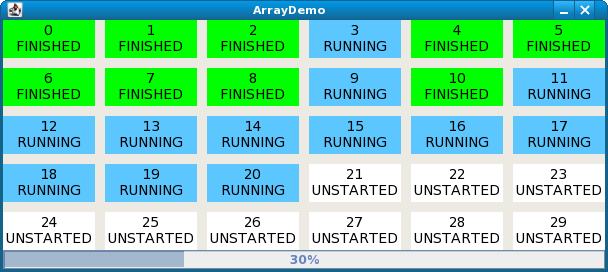
\includegraphics{images/array3_monitor}
\caption{Monitor dello stato di esecuzione del ``rendering'' di ogni gruppo di ``frame''.}
\label{fig:monitor-arraydemo}
\end{figure}
\item \label{lbl:exec-array3-postrenderstep1} Una volta che lo stato di esecuzione del ``rendering'' diventa \mgCode{FINISHED}, uscire dal programma digitando il valore $9$, seguito dal tasto \mgCode{Invio}, e, nuovamente, il valore $9$, seguito dal tasto \mgCode{Invio}.
\item \label{lbl:exec-array3-postrenderstep2} All'interno della cartella da cui \mgTheApp{} \`e stato eseguito, si troveranno $30$ file in formato ZIP:
\begin{mgCodeBox}
\small
array3.blend-rendered.zip\_1\_25\newline
array3.blend-rendered.zip\_26\_50\newline
array3.blend-rendered.zip\_51\_75\newline
array3.blend-rendered.zip\_76\_100\newline
array3.blend-rendered.zip\_101\_125\newline
array3.blend-rendered.zip\_126\_150\newline
array3.blend-rendered.zip\_151\_175\newline
array3.blend-rendered.zip\_176\_200\newline
array3.blend-rendered.zip\_201\_225\newline
array3.blend-rendered.zip\_226\_250\newline
array3.blend-rendered.zip\_251\_275\newline
array3.blend-rendered.zip\_276\_300\newline
array3.blend-rendered.zip\_301\_325\newline
array3.blend-rendered.zip\_326\_350\newline
array3.blend-rendered.zip\_351\_375\newline
array3.blend-rendered.zip\_376\_400\newline
array3.blend-rendered.zip\_401\_425\newline
array3.blend-rendered.zip\_426\_450\newline
array3.blend-rendered.zip\_451\_475\newline
array3.blend-rendered.zip\_476\_500\newline
array3.blend-rendered.zip\_501\_525\newline
array3.blend-rendered.zip\_526\_550\newline
array3.blend-rendered.zip\_551\_575\newline
array3.blend-rendered.zip\_576\_600\newline
array3.blend-rendered.zip\_601\_625\newline
array3.blend-rendered.zip\_626\_650\newline
array3.blend-rendered.zip\_651\_675\newline
array3.blend-rendered.zip\_676\_700\newline
array3.blend-rendered.zip\_701\_725\newline
array3.blend-rendered.zip\_726\_737
\end{mgCodeBox}
\item \label{lbl:exec-array3-postrenderstep3} Scompattare ciascun file all'interno di una opportuna cartella; la scompattazione creer\`a la sotto-cartella \mgCode{array3.blend-rendered} in cui si troveranno i seguenti file:
\begin{mgCodeBox}
\small
0001.png\newline
0002.png\newline
\dots\newline
0737.png
\end{mgCodeBox}
\item \label{lbl:exec-array3-postrenderstep4} \`E ora possibile combinare i suddetti file in modo opportuno, per esempio con il comando:
\begin{mgCodeBox}
\small
ffmpeg -i \%04d.png array3.mpeg
\end{mgCodeBox}
In Fig.~\ref{fig:exec-array3} sono mostrati alcuni fotogrammi della scena.
\begin{figure}
\centering
\begin{tabular}{ccc}

\includegraphics[scale=0.17]{images/array3-1} &

\includegraphics[scale=0.17]{images/array3-2} &

\includegraphics[scale=0.17]{images/array3-3} \tabularnewline

\includegraphics[scale=0.17]{images/array3-4} &

\includegraphics[scale=0.17]{images/array3-5} &

\includegraphics[scale=0.17]{images/array3-6} \tabularnewline

\includegraphics[scale=0.17]{images/array3-7} &

\includegraphics[scale=0.17]{images/array3-8} &

\includegraphics[scale=0.17]{images/array3-9}
\end{tabular}
\caption{Alcuni fotogrammi della scena \emph{ArrayDemo}.}
\label{fig:exec-array3}
\end{figure}
\end{enumerate}
Si noti che, durante l'immissione dei dati relativi alla scena, non \`e necessario inserire tutte le informazioni; in particolare, quando si accetta il valore di default proposto da \mgTheApp{} , \`e possibile evitare di accedere alla relativa voce di menu.
Ne segue che, in questo esempio, i passi descritti ai punti \ref{lbl:exec-array3-startframe-useless}, \ref{lbl:exec-array3-startframe2-useless}, \ref{lbl:exec-array3-stepframe-useless} e \ref{lbl:exec-array3-stepframe2-useless} possono essere evitati.
Ci\`o non vale, per\`o, se la voce del menu \`e etichettata con il simbolo \mgCode{[*]} (come nel caso del file della scena), il quale indica che l'inserimento del valore \`e obbligatorio.

I passi \ref{lbl:exec-array3-postrenderstep1}, \ref{lbl:exec-array3-postrenderstep2}, \ref{lbl:exec-array3-postrenderstep3} e \ref{lbl:exec-array3-postrenderstep4} possono essere automatizzati eseguendo lo script \emph{images2movie.sh}:
\begin{mgCodeBox}
./images2movie.sh array3 png
\end{mgCodeBox}
dove il primo argomento (in questo caso \emph{array3}) rappresenta il nome del file della scena (senza l'estensione \emph{.blend}), mentre il secondo argomento (in questo caso \emph{png}) rappresenta il formato delle immagini prodotte dal ``rendering'' dei vari gruppi di ``frame''.
L'uso di questo script necessita che nel sistema siano installati gli applicativi \emph{ffmpeg} e \emph{ffplay}.
